\section{Rechnerarchitekturen}\label{sec:rechnerarchitekturen}

\subsection{Einführung}\label{subsec:einfuehrung}

\begin{defi}{Struktur}
    Unter der \emph{Struktur} einer Rechnerarchitektur versteht man die Art der Verknüpfung der verschiedenen Hardwarekomponenten eines Rechner miteinander.
    
    Sie ist in der Regel \emph{statisch}.
\end{defi}

\begin{defi}{Organisation}
    Die \emph{Organisation} einer Rechnerarchitektur steht für die zeitabhängigen Wechselwirkungen zwischen Komponenten und die Steuerung dieser Komponenten.
    
    Diese Wechselwirkungen können \emph{dynamisch} sein.
\end{defi}

\begin{defi}{Implementierung}
    Die \emph{Implementierung} einer Rechnerarchitektur bezeichnet die Ausgestaltung einzelner Bausteine.
    
    Sie gibt die \emph{Größe} eines Systems an.
\end{defi}

\begin{defi}{Leistung}
    \emph{Leistung} beschreibt das nach außen hin sichtbare Systemverhalten.
    
    Sie gibt die \emph{Geschwindigkeit} eines Systems an.
\end{defi}

\subsection{Von-Neumann-Rechner}\label{subsec:von-neumann-rechner}

\begin{defi}{Von-Neumann-Rechner}
    Der \emph{Von-Neumann-Rechner} besteht aus folgenden Werken:
    \begin{itemize}
        \item \emph{Eingabe- bzw. Ausgabewerk:}
              \begin{itemize}
                  \item Schnittstelle zur Außenwelt
              \end{itemize}
        \item \emph{Leitwerk:}
              \begin{itemize}
                  \item interpretiert Befehle
                  \item steuert Abläufe
              \end{itemize}
        \item \emph{Haupt- bzw. Arbeitsspeicher:}
              \begin{itemize}
                  \item Speicher für Daten \emph{und} Befehle
                  \item unterteilt in Zellen gleicher Größe geteilt, die durch fortlaufende Adressen identifiziert werden
              \end{itemize}
        \item \emph{Rechenwerk:}
              \begin{itemize}
                  \item führt arithmetische und logische Operationen aus
              \end{itemize}
    \end{itemize}
    
    Die Struktur des Rechners ist unabhängig von der Aufgabe, die er lösen soll.
    Hardware und Software sind voneinander \emph{getrennt}.
\end{defi}

\begin{defi}[Von-Neumann-Rechner]{Struktur}
    TODO: Bild
\end{defi}

\begin{defi}[Von-Neumann-Rechner]{Organisation}
    TODO: Bild
\end{defi}

\begin{defi}[Von-Neumann-Rechner]{Arbeitsweise}
    Die \emph{Von-Neumann-Architektur} erlaubt nacheinander (\emph{sequentiell}):
    
    \begin{itemize}
        \item das Lesen eines Befehlscode-Worts oder
        \item das Lesen eines Datenworts oder
        \item das Schreiben eines Datenworts.
    \end{itemize}
    
    Befehlscode-Lesen und Daten-Lesen und -Schreiben konkurrieren.
    
    Von der Folge kann durch bedingte und unbedingte Sprungbefehle abgewichen werden, die die Programmfortsetzung an einer anderen Zelle bewirken.
    
    Die Maschine benutzt Binärcodes, Zahlen werden dual dargestellt.
\end{defi}

\begin{defi}[Von-Neumann-Rechner]{Von-Neumann-Flaschenhals}
    Der \emph{Von-Neumann-Flaschenhals} der Von-Neumann-Architektur beschreibt Performance-Verringerungen von Prozessoren durch konkurrierende Daten- und Befehlscode-Zugriffe über einen gemeinsamen Bus.
\end{defi}

\begin{bonus}[Von-Neumann-Rechner]{Von-Neumann-Flaschenhals}
    % TODO: https://de.wikipedia.org/wiki/Von-Neumann-Architektur (Quelle)
    Weitergehend beschreibt der \emph{Von-Neumann-Flaschenhals} auch das für diesen Sachverhalt verantwortliche Konzept des \enquote{immer nur eine Sache auf einmal} (eng.: \enquote{one-word-at-a-time thinking}), also den expliziten, erzwungenen Sequentialismus durch den einzigen Bus, über den alle Aktionen laufen.
    
    % TODO: https://dl.acm.org/doi/10.1145/359576.359579 (Quelle)
    John Backus beschreibt 1977 den \emph{Von-Neumann-Flaschenhals} wie folgt:
    \begin{quotation}
        Surely there must be a less primitive way of making big changes in the store than by pushing vast numbers of words back and forth through the von Neumann bottleneck.
        Not only is this tube a literal bottleneck for the data traffic of a problem, but, more importantly, it is an intellectual bottleneck that has kept us tied to word-at-a-time thinking instead of encouraging us to think in terms of the larger conceptual units of the task at hand.
        Thus programming is basically planning and detailing the enormous traffic of words through the von Neumann bottleneck, and much of that traffic concerns not significant data itself, but where to find it.
    \end{quotation}
\end{bonus}

\subsection{Rechenleistung}\label{subsec:rechenleistung}

\begin{defi}[Leistungsmaß]{Clock-Rate}
    Die Taktfrequenz $f$ (engl. \emph{Clock-Rate}) misst die Anzahl der Takte oder Zyklen, die von der CPU pro Sekunde durchgeführt werden in \emph{Hertz} \emph{Hz} ($\SI{1}{\hertz} = \SI{1}{\per\second}$).
\end{defi}

\begin{defi}[Leistungsmaß]{FLOPS}
    % TODO: https://de.wikipedia.org/wiki/Floating_Point_Operations_Per_Second (Quelle)
    Gleitkommaoperationen pro Sekunde (engl. \emph{FLOPS}; \emph{Floating Point Operations Per Second}) ist ein Maß für die Leistungsfähigkeit von Computersystemen und bezeichnet die Anzahl der Gleitkommazahl-Operationen (Additionen oder Multiplikationen), die von ihnen pro Sekunde ausgeführt werden können.
    
    In Domänen wie der numerischen Simulation ist die FLOPS-Angabe ein aussagekräftiges Maß für die Leistungsfähigkeit eines Computersystems als die Angabe der Clock-Rate allein.
    
    FLOPS auf einem System mit einer einzelnen CPU können wie folgt berechnet werden:
    \[
        \si{\flops} = \si{\cores} \cdot \si{\cycles\per\second} \cdot \si{\flops\per\cycle}
    \]
    
    FLOPS können in verschiedener Präzision angegeben werden:
    \begin{itemize}
        \item \emph{Half Precision}: 16 Bit
        \item \emph{Single Precision}: 32 Bit
        \item \emph{Double Precision}: 64 Bit
        \item \emph{Quadruple Precision}: 128 Bit
    \end{itemize}
\end{defi}

\begin{example}[Leistungsmaß]{FLOPS}
    TODO
\end{example}

\begin{bonus}{Top500}
    \begin{itemize}
        \item Erstellung der Liste der 500 schnellsten Rechner der Welt (2x pro Jahr)
        \item Leistungskriterium: Benchmark-Programme aus dem Gebiet der linearen Algebra (Linpack)
    \end{itemize}
    Beispiel:\\
    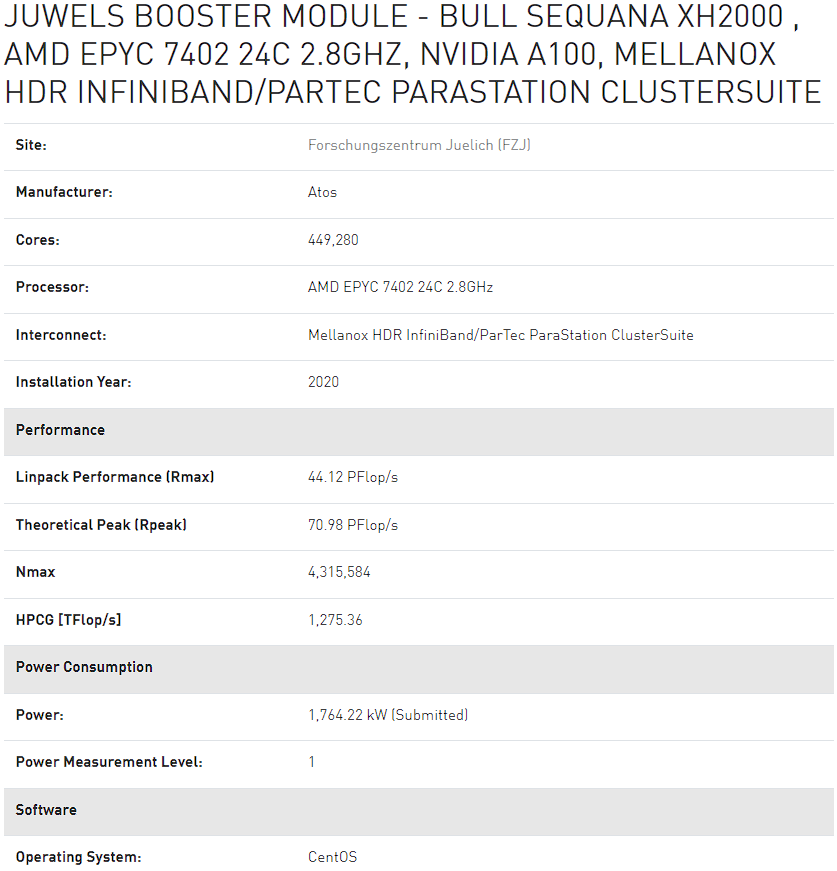
\includegraphics[width=\textwidth]{images/juwels_booster_top500.png}
    % TODO: Aus: Top500, \url{https://www.top500.org/system/179894/} Zuletzt aufgerufen am: 20.06.2023
\end{bonus}

\begin{bonus}{Transistoren und Clock-Rate}
    Die Weiterentwicklung bei der Chipherstellung (Lithographie) führt zu feineren Strukturen auf einem Chip.
    
    Was passiert, wenn Leiterbahnen und Schaltelemente um einen Faktor $x$ schrumpfen ?
    \begin{itemize}
        \item Clock-Rate $f$ wächst um Faktor $x$ (Stromverbrauch, Abwärme $T \sim f^2$)
        \item Die Anzahl der Transistoren pro Fläche wächst mit $x^2$
        \item Die Rechenleistung des Chips wächst mit $x^4$ (aber der Zuwachs um $x^3$ beruht auf Architektur)
    \end{itemize}
\end{bonus}

\begin{defi}{Moore's Law}
    % TODO: https://de.wikipedia.org/wiki/Mooresches_Gesetz (Quelle)
    \emph{Moore's Law} besagt, dass sich die Komplexität integrierter Schaltkreise mit minimalen Komponentenkosten regelmäßig verdoppelt; je nach Quelle werden 12, 18 oder 24 Monate als Zeitraum genannt.
    
    Unter Komplexität verstand Gordon Moore, der das Gesetz 1965 formulierte, die Anzahl der Schaltkreiskomponenten auf einem integrierten Schaltkreis. Gelegentlich ist auch von einer Verdoppelung der Integrationsdichte die Rede, also der Anzahl an Transistoren pro Flächeneinheit.
\end{defi}

\begin{bonus}[Moore's Law]{Verlauf bis 2011}
    % TODO: https://simple.wikipedia.org/wiki/Moore%27s_law (Quelle)
    \centering
    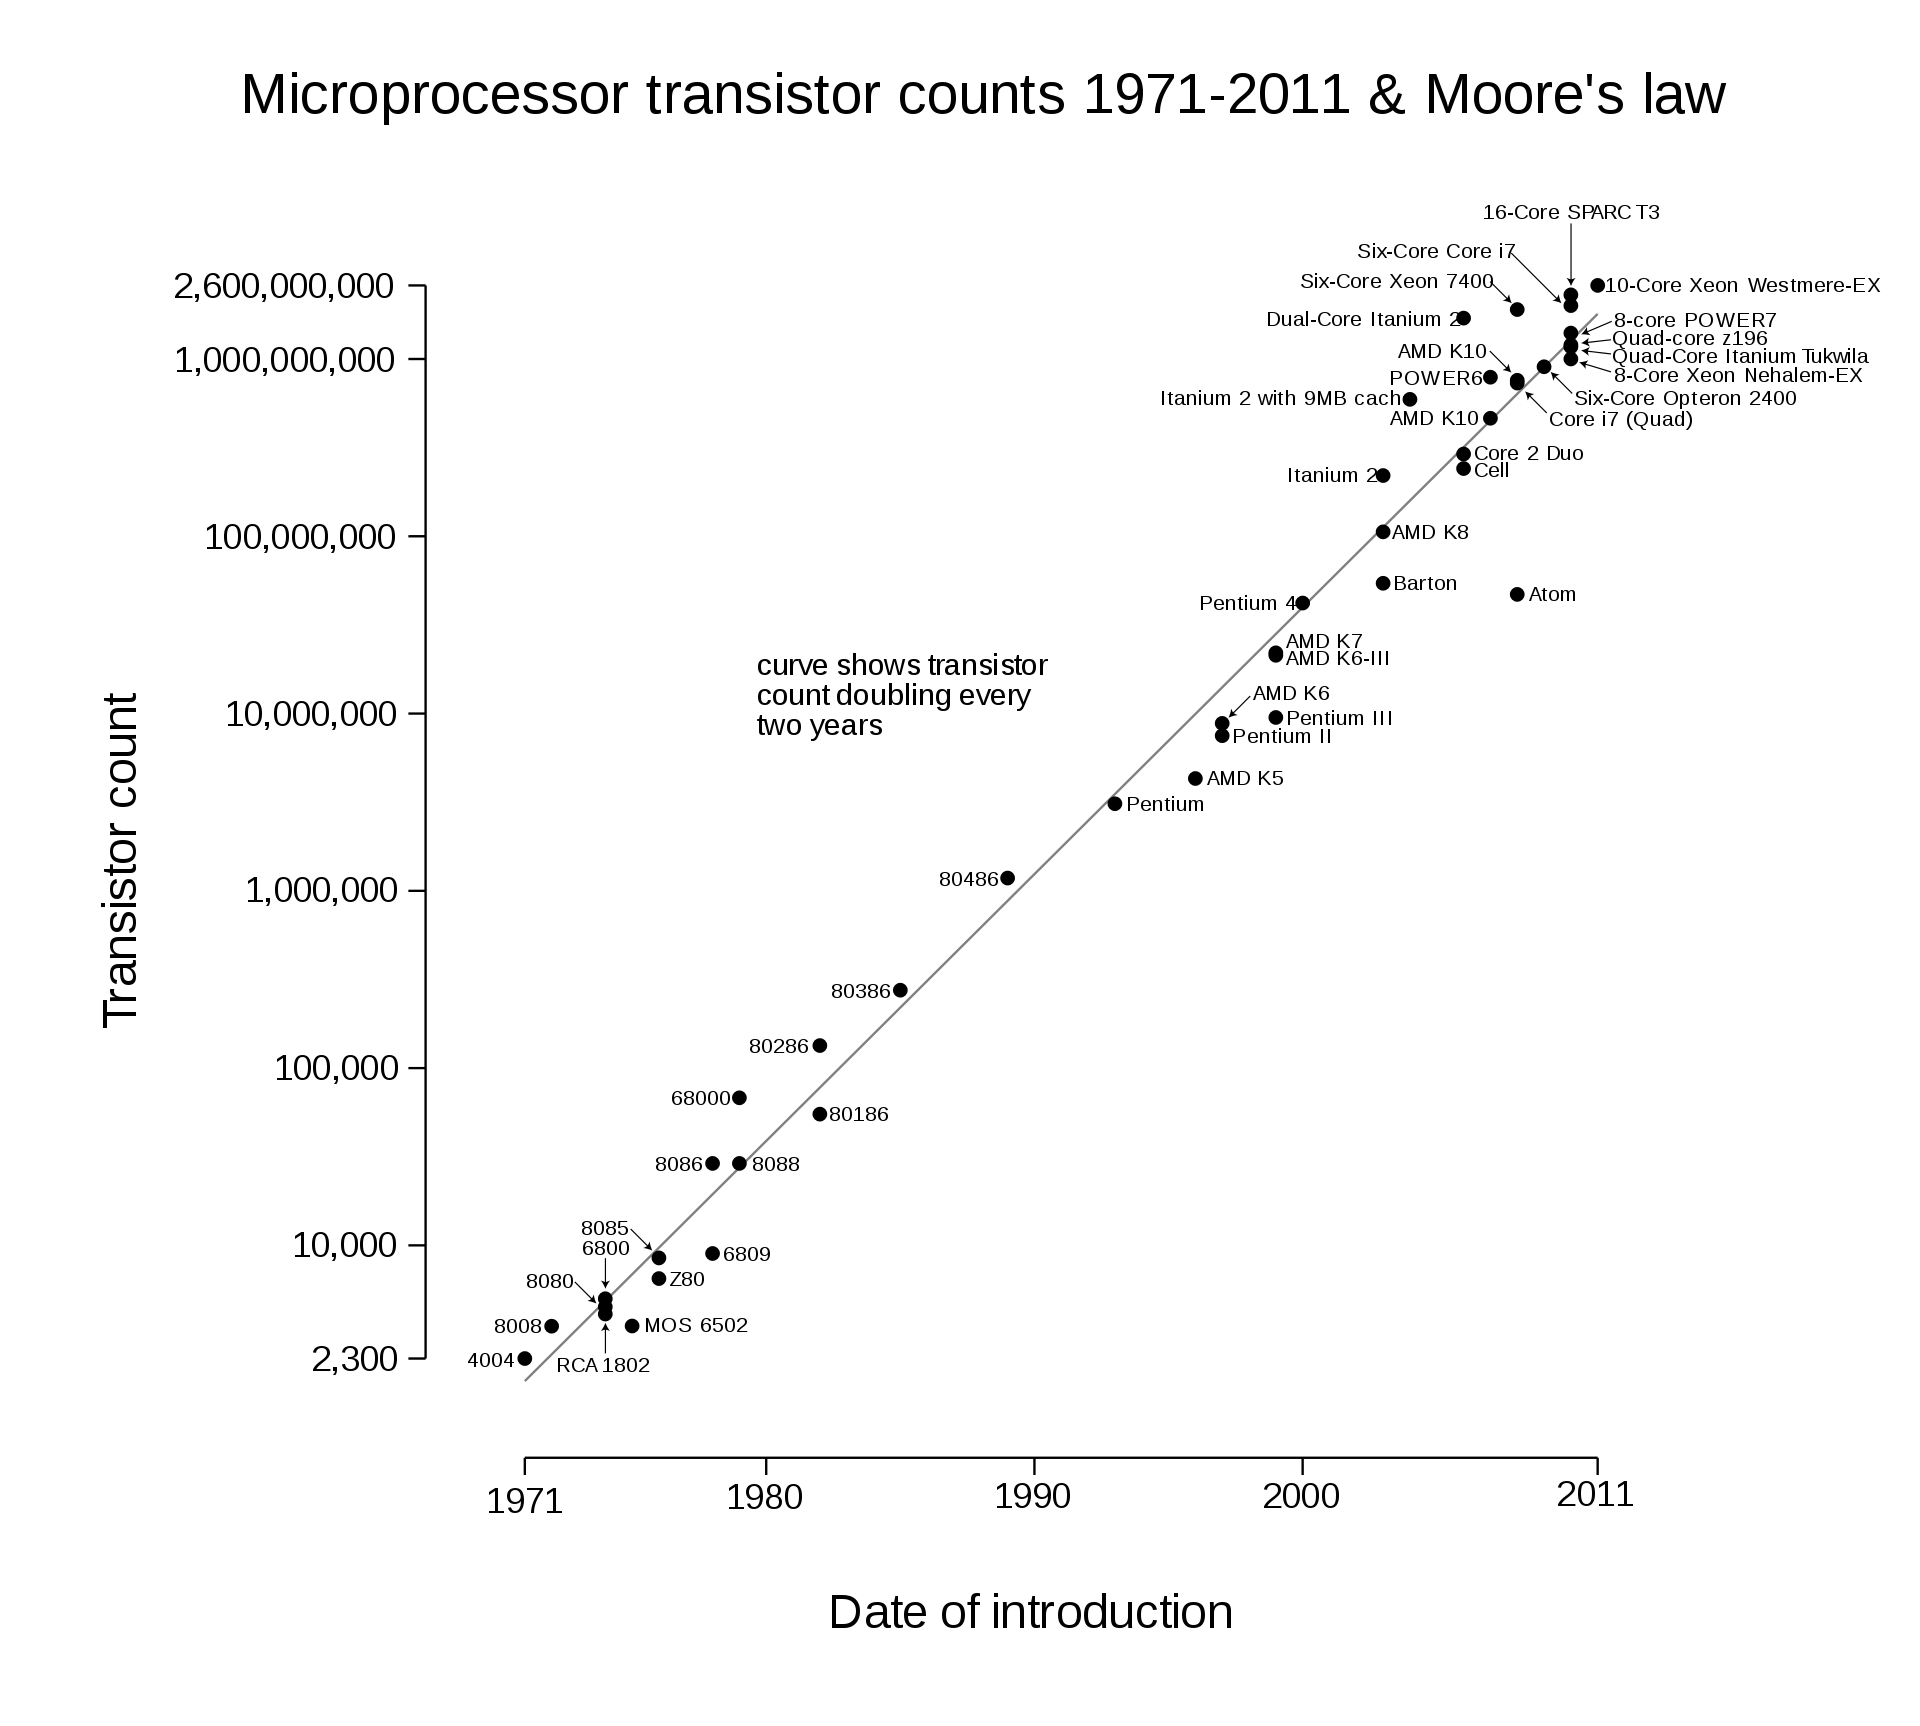
\includegraphics[width=0.75\textwidth]{images/moores_law.png}
\end{bonus}

\begin{bonus}{Leistungslücke Prozessor-Memory}
    Aufgrund von Moore's Law wächst die Leistungslücke (engl. \emph{Performance Gap}) um ca. 50\% pro Jahr, da bisher die CPU-Performance um ca. 60\% pro Jahr und die DRAM-Performance nur um ca. 7\% pro Jahr gewachsen ist.
    
    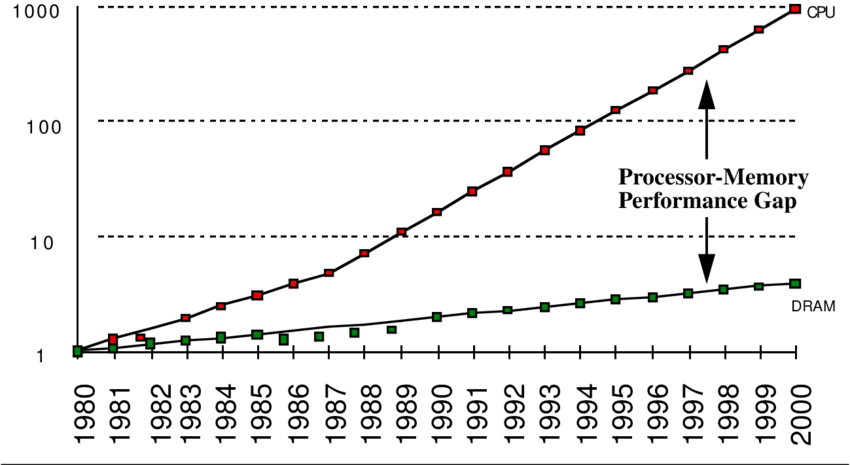
\includegraphics[width=\textwidth]{images/Processor-Memory-Performance-GapHen96.png}
    % TODO: Katherine Yelick, \url{https://www.researchgate.net/figure/Processor-Memory-Performance-GapHen96_fig1_3214931}, zuletzt aufgerufen am: 20.06.2023
\end{bonus}
